\documentclass[12pt,a4paper,oneside]{article}

\usepackage[utf8]{inputenc}
\usepackage[greek,english]{babel}
\usepackage{alphabeta} 

\usepackage[pdftex]{graphicx}
\usepackage[top=1in, bottom=1in, left=1in, right=1in]{geometry}
\usepackage{hyperref}
\linespread{1.06}
\setlength{\parskip}{8pt plus2pt minus2pt}
\usepackage{fancyhdr}
\widowpenalty 10000
\clubpenalty 10000

\newcommand{\eat}[1]{}
\newcommand{\HRule}{\rule{\linewidth}{0.5mm}}

\usepackage[official]{eurosym}
\usepackage{enumitem}
\setlist{nolistsep,noitemsep}
\usepackage[hidelinks]{hyperref}
 \usepackage[table]{xcolor}



\usepackage{lipsum}
\hypersetup{
    colorlinks=true,
    linkcolor=black,
    filecolor=magenta,      
    urlcolor=blue,
}

\begin{document}

\renewcommand{\contentsname}{Περιεχόμενα}

\renewcommand{\refname}{Αναφορές}

%===========================================================
\begin{titlepage}
\begin{center}

% Top 
\includegraphics[width=0.55\textwidth]{upatras_logo.jpg}~\\[2cm]


% Title
\HRule \\[0.4cm]
{ \LARGE 
  \textbf{PROJECT TΕΧΝΟΛΟΓΙΑ ΛΟΓΙΣΜΙΚΟΥ}\\[0.4cm]
  \emph{Project-plan-v0.1}\\[0.4cm]
}
\HRule \\[1.5cm]



% Author
{ \large
  \includegraphics[width=0.5\textwidth]{logo.png}~\\[2cm]
 
}

\vfill

\textsc{\large Τμήμα Μηχανικών Ηλεκτρονικών Υπολογιστών \& Πληροφορικής}\\[0.4cm]


% Bottom
{\large \selectlanguage{greek}\today}
 
\end{center}
\end{titlepage}
\pagestyle{fancy}
\fancyhead[RO,LE]{Project-plan-v0.1}
\fancyhead[LO,CE]{\includegraphics[width=0.05\textwidth]{logo.png}}
\centering
Ακολουθεί ο πίνακας με τα ονόματα και τα ΑΜ της ομαδάς μας:

\centering
\begin{tabular}{ |p{4cm}|p{4cm}|p{3cm}|}
\arrayrulecolor{gray}
 \hline
 \multicolumn{3}{|c|}{Μέλη} \\
 \hline
 ΕΠΩΝΥΜΟ& ΟΝΟΜΑ & Α.M\\
 \hline
 ΛΙΟΥΜΗΣ   & ΕΥΑΓΓΕΛΟΣ    & 1054325\\
 ΣΧΙΖΑΣ &  ΝΙΚΟΛΑΟΣ & 1054394\\
 ΛΥΡΟΥ & ΔΗΜΗΤΡΑ & 1057774\\
 ΜΠΟΥΡΣΑΛΗΣ   & ΕΜΜΑΝΟΥΗΛ & 1056284\\
\hline 

\end{tabular}


\vspace{7cm}
\raggedright
\textbf{Editors:}
\newline
Νίκος Σχίζας
\newlineΔήμητρα Λύρου
\newline
Ευάγγελος Λιούμης
\newline
Εμμανουήλ Μπούρσαλης


\vspace{7cm}

\raggedright
\textbf{Εργαλεία:}

    Overleaf
    
    Microsoft Visio(Pert Chart)
    
    TeamGantt(Gantt Chart)

\newpage

%===========================================================

\tableofcontents
\addtocontents{toc}{\protect\thispagestyle{empty}}

\newpage
\setcounter{page}{1}

%===========================================================
%===========================================================

\section{Gantt Chart}\label{sec:intro}
\pagestyle{fancy}
\fancyhead[RO,LE]{Project-plan-v0.1}
\fancyhead[LO,CE]{\includegraphics[width=0.05\textwidth]{logo.png}}
\textbf{Σημαντικές Διευκρινίσεις:}

\vspace{1mm}
Θεωρήσαμε ότι οι εργάσιμες ημέρες του έργου είναι Δευτέρα-Σάββατο. Παραβλέψαμε τις γραφειοκρατικές διαδικασίες για τη δημιουργία της επιχείρησης. Επίσης, θεωρήσαμε ότι κάθε 15 ημέρες γίνονται συνελεύσεις των ομάδων για αναφορά προόδου και ότι ο πελάτης είναι ένας επιβλέπων του κράτους και
όλη η επικοινωνία γίνεται με αυτόν. Επιπλέον, ορίσαμε ότι κάθε 10 ημέρες κατά το σχεδιασμό του
περιβάλλοντος διεπαφής χρήστη, της βάσης δεδομένων και της mobile εφαρμογής θα γίνονται αξιολογήσεις της μέχρι τότε πορείας του έργου. Υποθέσαμε ότι ήρθαμε σε επικοινωνία με το Υπουργείο Υγείας
και τους αναλύσαμε την ιδέα μας, τους κεντρίσαμε το ενδιαφέρον ώστε να φτάσουμε σε στάδιο διαγωνισμού για το έργο, το οποίο τελικά μας ανατέθηκε. Όσο να αφορά την μισθοδοσία των εργαζομένων της επιχείρησης είναι κοινή για όλους και ανέρχεται στα 10€/h. Θεωρούμε ότι δημιουργήθηκαν 4 ομάδες των 5 ατόμων με
επικεφαλής κάθε μίας, έναν από εμάς και ότι μέχρι την πρόσληψη του προσωπικού, δεν
πληρωνόμαστε.

 
\begin{center}

  \makebox[\textwidth]{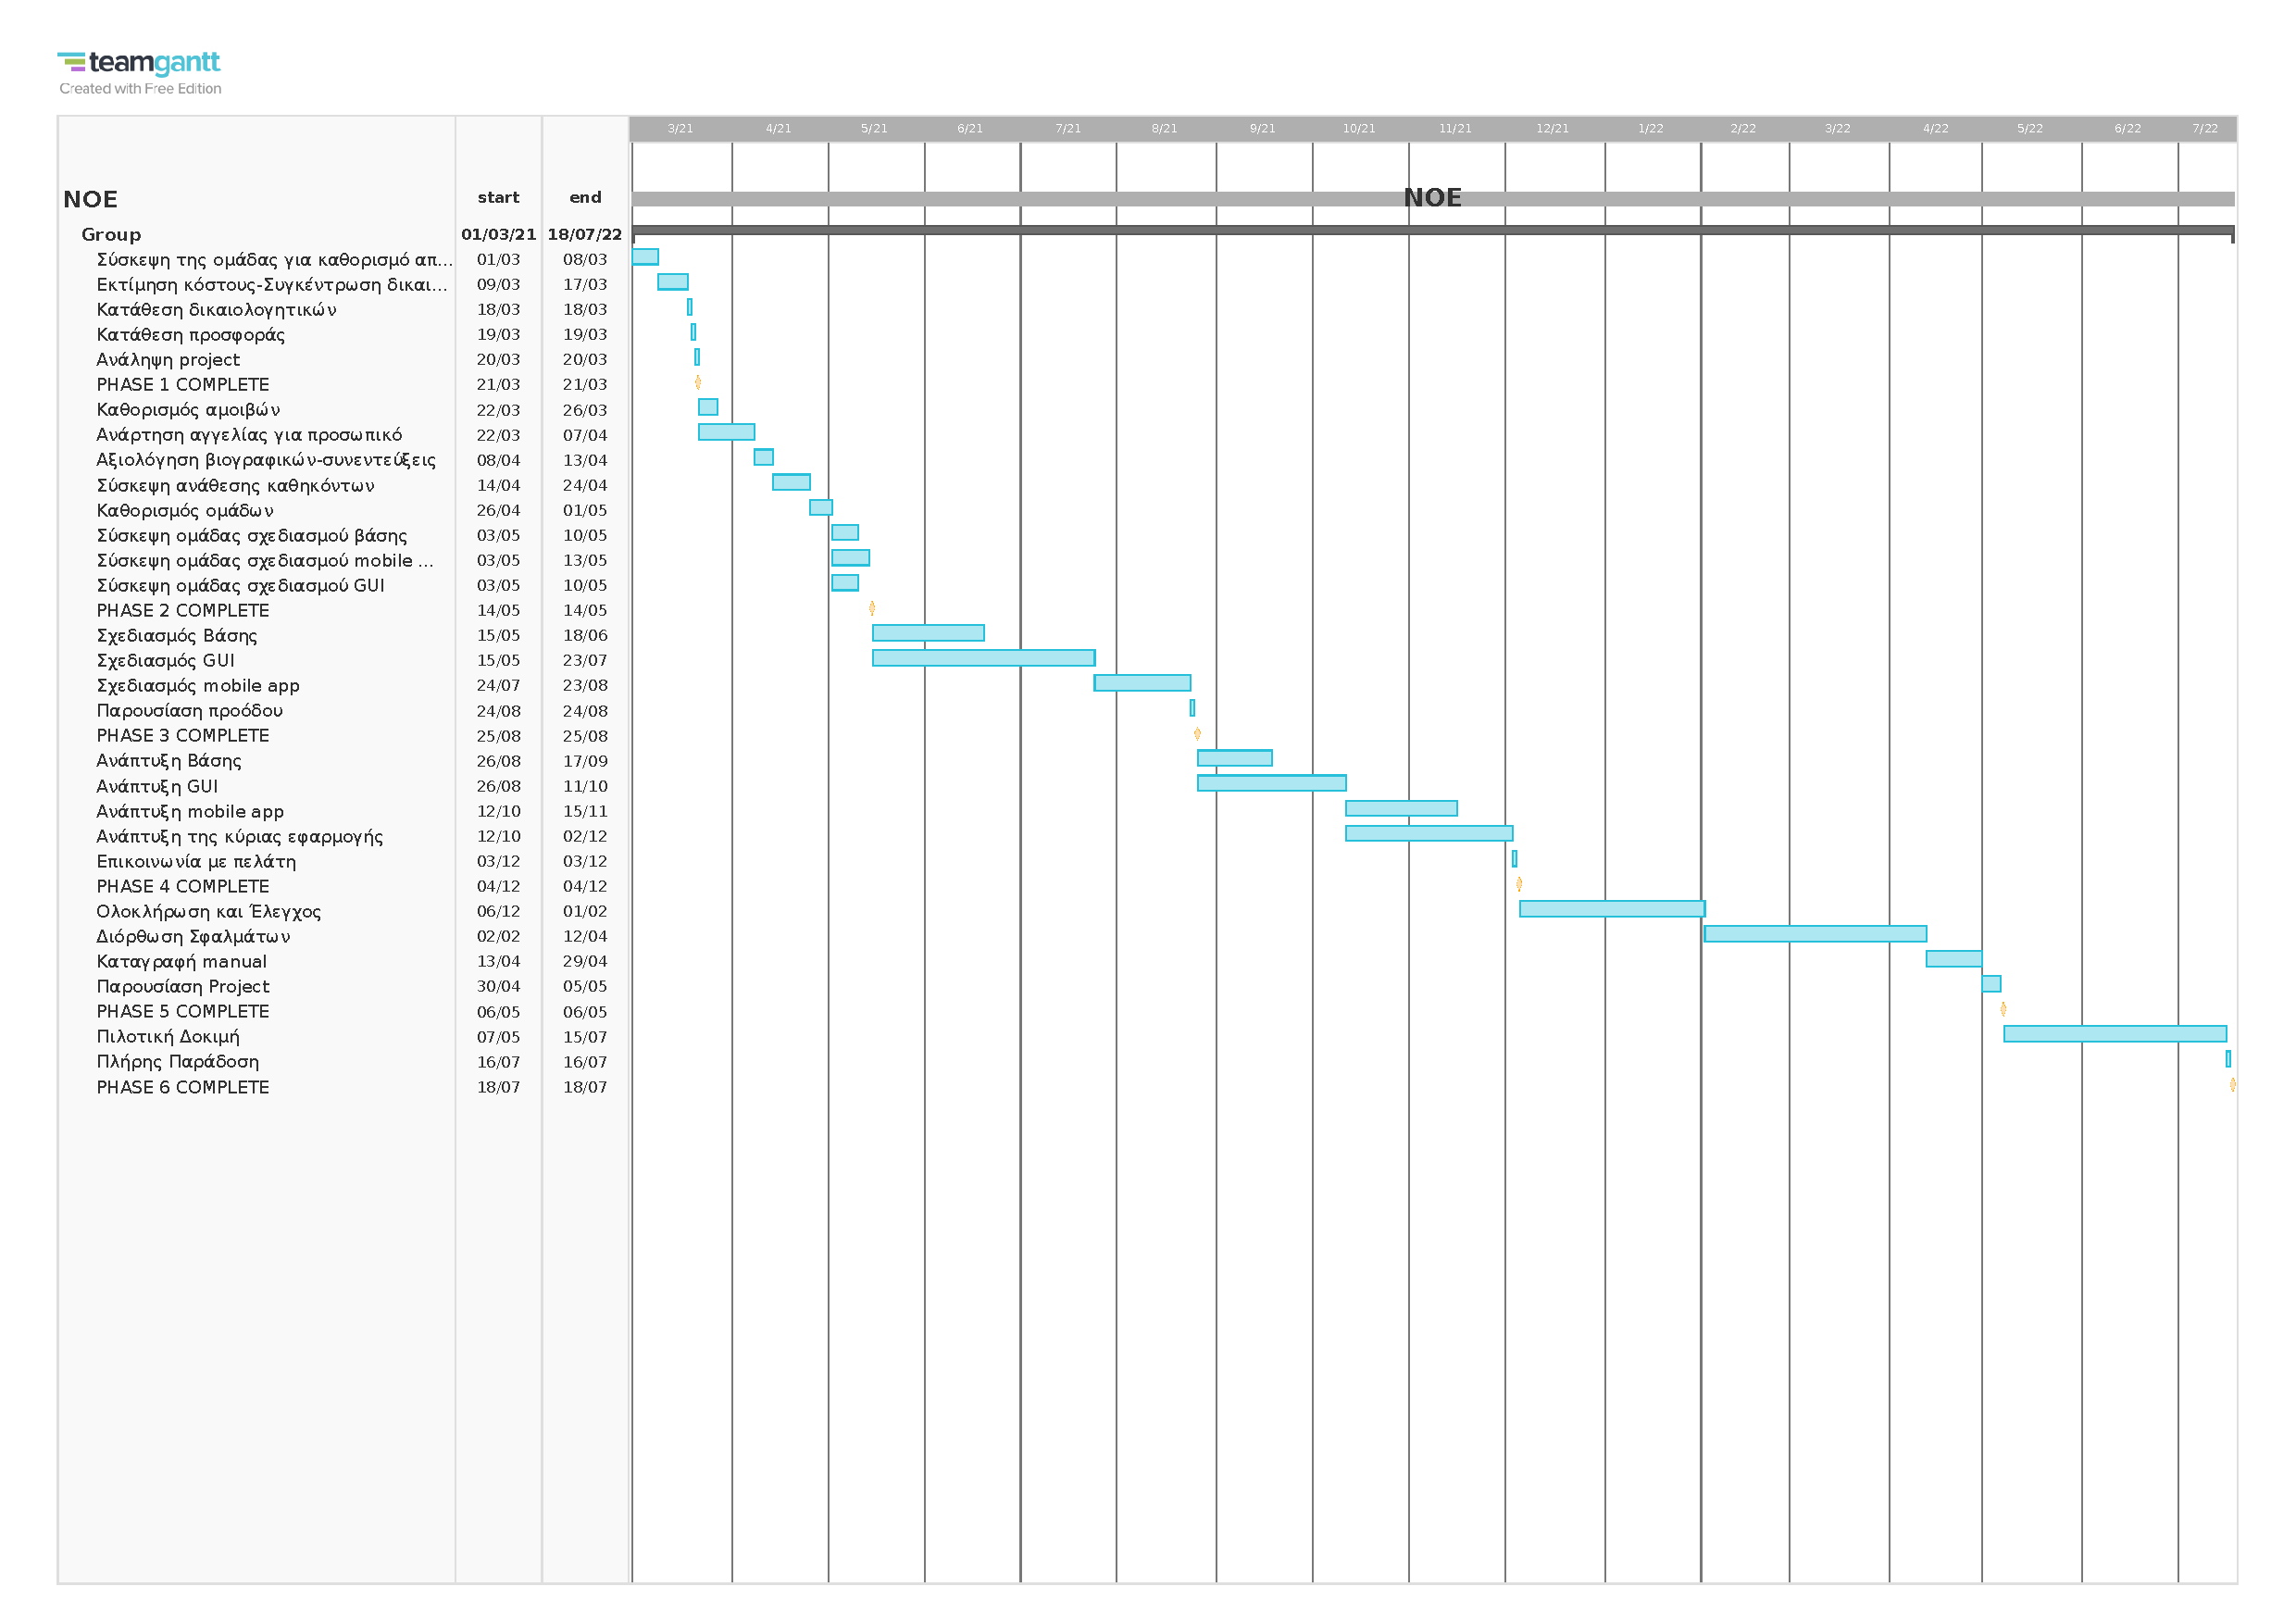
\includegraphics[width=1.35\textwidth]{NOE 3.pdf}}
    
\end{center}

\section{Pert Chart}\label{sec:lit-rev}


\centerline{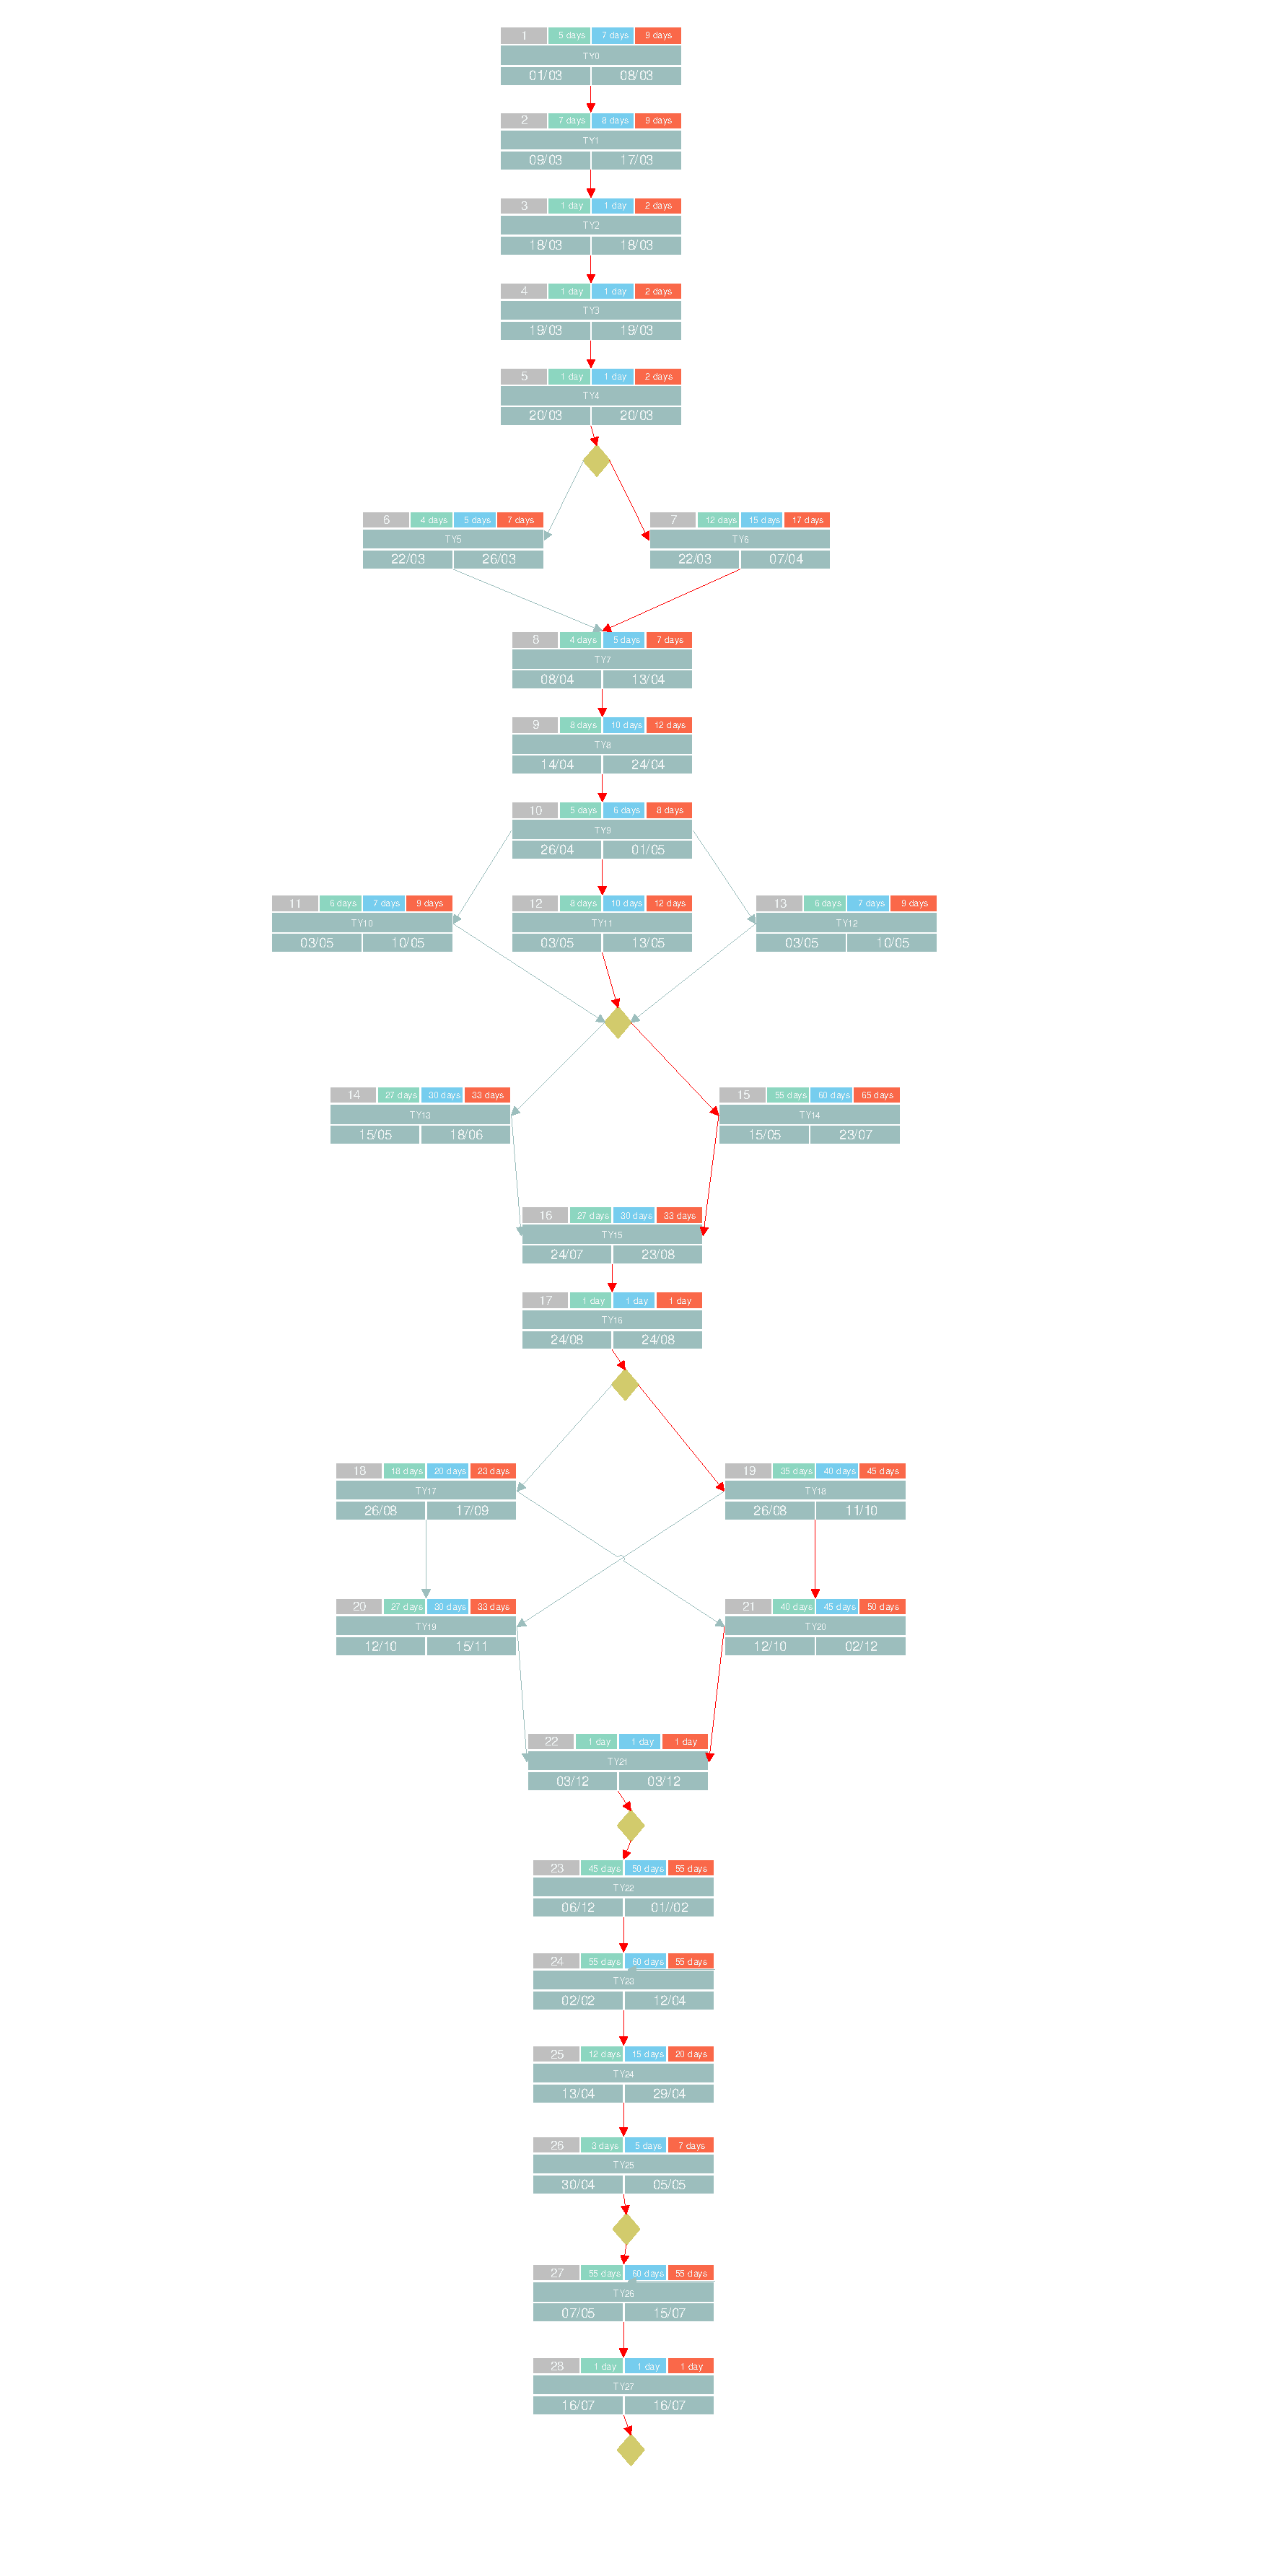
\includegraphics[width=17cm,height=23.7cm]{Pert plan.pdf}}


\newpage 
\section{Ανάθεση Έργου}\label{sec:meth}
Για ευκολία και επειδή στο Pert δεν μπορούσαν να προσθεθούν κατάλληλα τα ονόματα των μελών μας επιλέξαμε ένα γράμμα που αντιστοιχεί στα ονομάτα(ΔΗΜΗΤΡΑ ΛΥΡΟΥ--\textgreaterΔ, ΕΜΜΑΝΟΥΗΛ ΜΠΟΥΡΣΑΛΗΣ--\textgreaterΜ, ΝΙΚΟΛΑΟΣ ΣΧΙΖΑΣ--\textgreaterΝ, ΕΥΑΓΓΕΛΟΣ ΛΙΟΥΜΗΣ--\textgreaterΒ.)Πιο επεξηγηματικά η αντιστοίχιση φαίνεται στον παρακάτω πίνακα:

\begin{tabular}{ |p{4cm}|p{6cm}|p{4cm}|}
\arrayrulecolor{gray}
 \hline
 
 \hline
 \textbf{ΤΥ} & \textbf{Τίτλος} & \textbf{Ανθρώπινο Δυναμικό}\\
 \hline
ΤΥ0 & Σύσκεψη της ομάδας για καθορισμό απαιτήσεων & Δ Μ Ν Β\\
\hline
ΤΥ1 & Εκτίμηση Κόστους-Συγκέντρωση Δικαιολογητικών & Ν Β\\
\hline
ΤΥ2 & 	Κατάθεση Δικαιολογητικών & Μ\\
\hline
ΤΥ3 & Κατάθεση προσφοράς & Δ\\
\hline
ΤΥ4 & Ανάληψη project &	Δ Μ Ν Β\\
\hline
ΤΥ5 & Καθορισμός αμοιβών &	Δ Ν\\
\hline
ΤΥ6 & Ανάρτηση αγγελίας για προσωπικό & Μ Β\\ 
\hline
ΤΥ7 &Αξιολόγηση βιογραφικών-συνεντεύξεις&Δ Μ Ν Β \\
\hline
ΤΥ8 & Σύσκεψη ανάθεσης καθηκόντων&Δ Μ Ν Β\\
\hline
ΤΥ9 & Καθορισμός ομάδων&Δ Μ Ν Β\\
\hline
ΤΥ10 & Σύσκεψη ομάδας σχεδιασμού βάσης&Δ\\
\hline
ΤΥ11 & Σύσκεψη ομάδας σχεδιασμού mobile εφαρμογής&Μ Ν\\
\hline
ΤΥ12 &Σύσκεψη ομάδας σχεδιασμού GUI	&Β\\
\hline
ΤΥ13 &Σχεδιασμός Βάσης&Μ Ν\\
\hline
ΤΥ14 &	Σχεδιασμός GUI&Δ Β\\
\hline
ΤΥ15 & Σχεδιασμός mobile app&Δ Μ Ν Β\\
\hline
ΤΥ16 & Παρουσίαση προόδου&Δ Μ Ν Β\\
\hline
ΤΥ17 &Ανάπτυξη Βάσης&Δ Β\\
\hline
ΤΥ18 & Ανάπτυξη GUI	&Μ Ν\\
\hline
ΤΥ19 & Ανάπτυξη mobile app&Μ Ν\\
\hline
ΤΥ20 & Ανάπτυξη της κύριας εφαρμογής&Δ Β\\
\hline
ΤΥ21 & Επικοινωνία με πελάτη&Δ Μ Ν Β\\
\hline
ΤΥ22 & Ολοκλήρωση και Έλεγχος&Δ Μ Ν Β\\
\hline
ΤΥ23 & Διόρθωση Σφαλμάτων&Δ Μ Ν Β\\
\hline
ΤΥ24 & Καταγραφή manual&Δ Μ Ν Β\\
\hline
ΤΥ25 & Παρουσίαση Project&Δ Μ Ν Β\\
\hline
ΤΥ26 & Πιλοτική Δοκιμή&Δ Μ Ν Β\\
\hline
ΤΥ27 &Πλήρης Παράδοση&Ν\\
\hline 

\end{tabular}
\newpage

\section{Εκτίμηση Κόστους}\label{sec:res}
Παρακάτω φαίνεται ο πίνακας με τα Άμεσα και Έμμεσα κόστη που θεωρούμε ότι θα υπάρξουν καθώς και ένα γράφημα για καλύτερη αναπαράσταση τους για το έργου μας:
\centerline{\includegraphics[page=1,width=1.05\textwidth]{Βιβλίο1 (version 1) (1)-converted.pdf}}


\newpage

%===========================================================
%===========================================================
\addcontentsline{toc}{section}{Αναφορές}
\bibliographystyle{ieeetr}
\bibliography{refs}


\end{document} 
